\documentclass[journal]{vgtc}                % final (journal style)
%\documentclass[review,journal]{vgtc}         % review (journal style)
%\documentclass[widereview]{vgtc}             % wide-spaced review
%\documentclass[preprint,journal]{vgtc}       % preprint (journal style)

%% Uncomment one of the lines above depending on where your paper is
%% in the conference process. ``review'' and ``widereview'' are for review
%% submission, ``preprint'' is for pre-publication, and the final version
%% doesn't use a specific qualifier.

%% Please use one of the ``review'' options in combination with the
%% assigned online id (see below) ONLY if your paper uses a double blind
%% review process. Some conferences, like IEEE Vis and InfoVis, have NOT
%% in the past.

%% Please use the ``preprint''  option when producing a preprint version
%% for sharing your article on an open access repository

%% Please note that the use of figures other than the optional teaser is not permitted on the first page
%% of the journal version.  Figures should begin on the second page and be
%% in CMYK or Grey scale format, otherwise, colour shifting may occur
%% during the printing process.  Papers submitted with figures other than the optional teaser on the
%% first page will be refused. Also, the teaser figure should only have the
%% width of the abstract as the template enforces it.

%% These few lines make a distinction between latex and pdflatex calls and they
%% bring in essential packages for graphics and font handling.
%% Note that due to the \DeclareGraphicsExtensions{} call it is no longer necessary
%% to provide the the path and extension of a graphics file:
%% \includegraphics{diamondrule} is completely sufficient.
%%
\ifpdf%                                % if we use pdflatex
  \pdfoutput=1\relax                   % create PDFs from pdfLaTeX
  \pdfcompresslevel=9                  % PDF Compression
  \pdfoptionpdfminorversion=7          % create PDF 1.7
  \ExecuteOptions{pdftex}
  \usepackage{graphicx}                % allow us to embed graphics files
  \DeclareGraphicsExtensions{.pdf,.png,.jpg,.jpeg} % for pdflatex we expect .pdf, .png, or .jpg files
\else%                                 % else we use pure latex
  \ExecuteOptions{dvips}
  \usepackage{graphicx}                % allow us to embed graphics files
  \DeclareGraphicsExtensions{.eps}     % for pure latex we expect eps files
\fi%

%% it is recomended to use ``\autoref{sec:bla}'' instead of ``Fig.~\ref{sec:bla}''
\graphicspath{{figures/}{pictures/}{images/}{./}} % where to search for the images

\usepackage{microtype}                 % use micro-typography (slightly more compact, better to read)
\PassOptionsToPackage{warn}{textcomp}  % to address font issues with \textrightarrow
\usepackage{textcomp}                  % use better special symbols
\usepackage{mathptmx}                  % use matching math font
\usepackage{times}                     % we use Times as the main font
\renewcommand*\ttdefault{txtt}         % a nicer typewriter font
\usepackage{cite}                      % needed to automatically sort the references
\usepackage{tabu}                      % only used for the table example
\usepackage{booktabs}                  % only used for the table example
\usepackage{amsfonts}
\usepackage{amsmath, algpseudocode}
\usepackage{algorithm, algorithmicx}
%% We encourage the use of mathptmx for consistent usage of times font
%% throughout the proceedings. However, if you encounter conflicts
%% with other math-related packages, you may want to disable it.

%% In preprint mode you may define your own headline. If not, the default IEEE copyright message will appear in preprint mode.
%\preprinttext{To appear in IEEE Transactions on Visualization and Computer Graphics.}

%% In preprint mode, this adds a link to the version of the paper on IEEEXplore
%% Uncomment this line when you produce a preprint version of the article 
%% after the article receives a DOI for the paper from IEEE
%\ieeedoi{xx.xxxx/TVCG.201x.xxxxxxx}

%% If you are submitting a paper to a conference for review with a double
%% blind reviewing process, please replace the value ``0'' below with your
%% OnlineID. Otherwise, you may safely leave it at ``0''.
\onlineid{0}

%% declare the category of your paper, only shown in review mode
\vgtccategory{Research}
%% please declare the paper type of your paper to help reviewers, only shown in review mode
%% choices:
%% * algorithm/technique
%% * application/design study
%% * evaluation
%% * system
%% * theory/model
\vgtcpapertype{please specify}


\newcommand{\stitle}[1]{\vspace*{0.4em}\noindent{\bf #1:\/}}
\newcommand{\sstitle}[1]{\vspace*{0.4em}\noindent{\bf #1\/.}}
\newcommand{\DQV}{\mathsf{QEVIS}}


\newcommand{\QM}[1]{{\color{blue}{#1}}}
%% Paper title.
\title{$\DQV$: Understanding and Diagnosing the Fine-grained Execution Process of Hive Query via Visualization}

%% This is how authors are specified in the journal style

%% indicate IEEE Member or Student Member in form indicated below
% \author{Roy G. Biv, Ed Grimley, \textit{Member, IEEE}, and Martha Stewart}
% \authorfooter{
% %% insert punctuation at end of each item
% \item
%  Roy G. Biv is with Starbucks Research. E-mail: roy.g.biv@aol.com.
% \item
%  Ed Grimley is with Grimley Widgets, Inc.. E-mail: ed.grimley@aol.com.
% \item
%  Martha Stewart is with Martha Stewart Enterprises at Microsoft
%  Research. E-mail: martha.stewart@marthastewart.com.
% }

%other entries to be set up for journal
% \shortauthortitle{Biv \MakeLowercase{\textit{et al.}}: Global Illumination for Fun and Profit}
%\shortauthortitle{Firstauthor \MakeLowercase{\textit{et al.}}: Paper Title}

%% Abstract section.
\abstract{
Understanding the query execution process of distributed databases is crucial to many real-world practices such as detecting query bottlenecks and improving system performance. However, analyzing distributed query execution is challenging due to a large number of parallel tasks and the complex dependencies among these tasks. Moreover, system statuses such as network and memory can also affect query execution in complicated ways. Existing techniques typically collect \textit{aggregate statistics} of system performance (e.g., CPU, memory, and disk I/O) or execution progress (e.g., operator duration), and thus cannot track \textit{fine-grained query execution process} at the atomic task level, which is key to reason the query behavior. To tackle this problem, we propose $\DQV$, a visual analytics system that supports understanding and diagnosing distributed query execution from multiple views in an interactive manner. We tailor-make an algorithm for temporal directed acyclic graph (TDAG) layout to visualize the overall structure and execution process of the query plan. A suite of novel visualization and interaction designs are introduced to analyze the tasks, data dependency, and relation between atom task execution and system performance metrics. We illustrate the effectiveness of our $\DQV$ with three real-world case studies (i.e., query optimization, system configuration and xxx) and interviews with domain experts.

%Understanding the query execution of distributed databases is crucial to many real-world practices such as detecting the query bottleneck and improving the system performance.  Such analysis is always challenging due to the large volume of tasks executed in parallel and the complex task dependencies. Moreover, the unpredicted system behaviors also affect the query execution case by case. Existing techniques usually evaluate the distributed query by the statistics of system performance (e.g., CPU, memory, and disk I/O) or execution metrics(e.g., operator duration), which lost the fine-grained information at the atom task level. To tackle this problem, we propose $\DQV$, a visual analytics system to interactively understand and diagnose the distributed query execution procedure from multiple levels. An optimized algorithm for the temporal directed acyclic graph(TDAG) layout is devised to show the overall query plan structure and execution process. A suite of novel visualization and interaction designs are integrated to estimate the correlation between the atom task trace and the system performance metrics.  We illustrate the effectiveness of our $\DQV$ with three case studies from real-world applications and interviews with domain experts.
} 
% end of abstract

%% Keywords that describe your work. Will show as 'Index Terms' in journal
%% please capitalize first letter and insert punctuation after last keyword
\keywords{Radiosity, global illumination, constant time}

%% ACM Computing Classification System (CCS). 
%% See <http://www.acm.org/class/1998/> for details.
%% The ``\CCScat'' command takes four arguments.

\CCScatlist{ % not used in journal version
 \CCScat{K.6.1}{Management of Computing and Information Systems}%
{Project and People Management}{Life Cycle};
 \CCScat{K.7.m}{The Computing Profession}{Miscellaneous}{Ethics}
}

%% A teaser figure can be included as follows
\teaser{
  \centering
  \includegraphics[width=\linewidth]{figures/teaser/systemview.png}
  \caption{In the Clouds: Vancouver from Cypress Mountain. Note that the teaser may not be wider than the abstract block.}
  \label{fig:teaser}
}

%% Uncomment below to disable the manuscript note
%\renewcommand{\manuscriptnotetxt}{}

%% Copyright space is enabled by default as required by guidelines.
%% It is disabled by the 'review' option or via the following command:
% \nocopyrightspace


\vgtcinsertpkg

%%%%%%%%%%%%%%%%%%%%%%%%%%%%%%%%%%%%%%%%%%%%%%%%%%%%%%%%%%%%%%%%
%%%%%%%%%%%%%%%%%%%%%% START OF THE PAPER %%%%%%%%%%%%%%%%%%%%%%
%%%%%%%%%%%%%%%%%%%%%%%%%%%%%%%%%%%%%%%%%%%%%%%%%%%%%%%%%%%%%%%%%

\begin{document}

%% The ``\maketitle'' command must be the first command after the
%% ``\begin{document}'' command. It prepares and prints the title block.

%% the only exception to this rule is the \firstsection command

\firstsection{Introduction}
\maketitle

The distributed database system is becoming increasingly pervasive due to the explosive growth of data in science, industrial and life.
Meanwhile, many tools such as Hive, Flink and Vertical are developed to optimize the query, translate traditional query language to execution plan based on the map-reduce framework and dispatch multiple tasks to clusters to perform the data acquisition in parallel.

To maximally leverage the distributed systems, it is crucial for users to understand and evaluate how the query runs across the clusters. The frequently asked questions include "Where does the time go?", "What is the bottleneck of my query?", "Can we improve the performance of the specific query?".  Many research work devoted to evaluating and improving the performance of data analytic frameworks, but most of them try to reveal the performance by making high-level statistics about the correlated metrics collected from the accumulated logs or experiment conducted on benchmarks, which cannot be used for the understanding of the special case and provide the details answer for these questions. Specific methods which can look into the query execution process are required.

Understanding query logic and execution in the distributed environment is challenging. Three stages are involved for human-beings to understand a database query comprehensively: 1) understand the query logic, 2) understand the execution plan structure, and 3) understand the plan execution procedure.
Understand the query logic itself is long studied direction, especially when the queries are becoming increasing deep and nested.
With the pervasive of distributed database system, visual explaining of distributed execution plan structure is studied. These methods transform the abstract execution plan with thousands of lines of description to intuitive diagrams such as tree or graph and design interactions allowing users to interactively explore the nested structures.
In our paper, we mainly focus on the stage 3) i.e. understand the execution procedure of query execution.There are three challenges to facilitate the fine-grained analysis of query executions.

\stitle{Large number of atom tasks}
When issuing the execution plan on the distributed database system, large number of atomic tasks will be generated and executed on the nodes in the cluster in parallel. The duration of tasks may be significant different from each other even executed on the same server. Identifying the unnature long cases and analyzing their performance from the large amount of tasks is challenges, since it is difficult to define clear ground truth to fits all cases.

\stitle{Complex dependencies among the tasks}
The processing of a task always depends on several prerequisite tasks which provide the necessary input data. Analyzing the complex many to many dependencies and identifying the trace of interested are difficult in the large task set.

\stitle{Unpredicted behavior of distributed system} also increases he difficulty to understand the model execution procedure. For instance, the developer find that the same query execution plan run today may be different from that of yesterday. In general, four aspects are considered to affect the performance of clusters: CPU usage, memory usage, network IO and disk status. Existing work studies try to reveal how these metrics related to the system performance or quantify the impact and significance of these features. These studies are conducted based on the observed performance data from the experiment or logs collected from the production environment. One work inspired us is $\DQV$ which tries to linkage the resources status to query performance and resource usages. However, these work fail to provide the fine-grained execution traces for users to inspect the reasons of model behavior.
% There are three challenges to facilitate the fine-grained inspection of query executions. 
% \textbf{Non-transparent translation} makes it difficult for database users to inspect the query behaviors for a given abstract query. As shown by Figure**, the query issued by users is highly abstract which hides the detailed executed logic on a distributed system. The tools such as Hive can translate the query to a physical execution plan as shown by Figure~\ref{fig:exec_plan}. The execution plans have hundreds to thousands of lines of description, which is difficult for users to build a mental map for the overall execution plan. Existing work tries to bridge the gap between the execution logic and human perception by visualizing the execution plan as directed acyclic graph and allow users to interactively narrow down to any detailed operator as demand. However, the visualization of execution plan is always independent from the visualization of execution process. During the exploration, the users have to switch between multiple views which break the continuity of the plan-execution analysis.
% \textbf{Unexpected behavior of distributed system} also increases he difficulty to understand the model execution process. For instance, the developer find that the same query execution plan run today may be different from that of yesterday. In general, four aspects are considered to affect the performance of clusters: CPU usage, memory usage, network IO and disk status. Existing work studies try to reveal how these metrics related to the system performance or quantify the impact and significance of these features. These studies are conducted based on the observed performance data from the experiment or logs collected from the production environment. One work inspired us is $\DQV$ which tries to linkage the resources status to query performance and resource usages. However, these work fail to provide the fine-grained execution traces for users to inspect the reasons of model behavior.

In this work, we develop a visual analytics system called $\DQV$ (Figure~\ref{fig:teaser}) for database users to monitor, understand and diagnose query behavior across the distributed system. The system can be run with three modes: 1) monitoring mode: the system runs with the query execution process, collects and visualizes the query status in real-time; 2) simulation mode: the system will replay the execution process with given simulation rate; 3) analysis mode: the system will directly show the final results for users to explore the final results. In the visualization component, we design a temporal DAG (directed acyclic graph) diagram to display the execution plan and execution process dynamically and seamlessly. To enable the scalable visual analysis of the large number of tasks executed on the computing nodes, we implement the compound trace diagram which integrates the point cloud form and progress bar form together to meet the different analysis requirements. The monitoring results are visualized in the monitoring view and linked with the other analysis views through a suit of flexible interactions. 


%% \section{Introduction} %for journal use above \firstsection{..} instead
\begin{itemize}
% \item A framework to systematically analyze the query execution on distributed database by integrating three components: query analyzing component, machine monitoring component and analytic component.
\item The design and implementation of $\DQV$, a visual analytic system for understanding and analyzing the distributed query execution process.
\item Well-established visualization front-end to support the interactive investigating, comparing and diagnosing the query process. The system includes a set of novel designs for visualizing the temporal DAG and sequence group.
\item Case studies on the analysis of query process performed on the Hadoop platform.
\end{itemize}

\section{Related work}
\subsection{Visual Analysis for Database Queries}
%Understanding the query behavior and evaluating database performance has been studied for decades since the database management systems(DBMSs) have been found. Both database and visualization communities have proposed methods to analyze the performance and diagnose the queries automatically or manually. We give a brief introduction about the related works from the two following aspects: \textit{query logic structure} and \textit{query execution structure}, and refer the interested readers to~\cite{gathani2020debugging} for the systematic overview about the database query debug and performance analysis.


%Understanding query performance has long been studied since the advent of database management systems (DBMSs). 

Both the database and visualization communities have proposed methods to analyze query performance and diagnose performance problems manually or automatically. We briefly review related works on \textit{understanding query logic} and \textit{analyzing query execution plan}, and refer the interested readers to~\cite{gathani2020debugging} for a systematic survey on database query debugging and performance analysis.

%\emph{\textbf{Analyzing query structure}}. Queries such as SQL sentences can be hard to read since they always have a deep and nested structure. Many research works have been conducted to help the database users to understand the quires quickly. The most common method is to utilize visualization techniques to show the logic structure of operations[all]. For example, extended from previous work, QueryVis uses the node-link diagrams to show the relationship between operators; the unambiguity is also proved in this paper. Other than visualization, Gawade et al. proposed a method to translate a query to Natural Language.  


\emph{\textbf{Understand query logic}}. Query specifications in high-level languages such as SQL can be difficult to read as they may have deep and nested structures. Many research works have tried to provide an intuitive understanding of the query logic~\cite{abouzied2012dataplay, gatterbauer2011databases, cerullo2007system,jaakkola2003visual,leventidis2020queryvis,danaparamita2011queryviz}. 
The most common way is to leverage visualization techniques to assist query understanding.
For example, GraphSQL~\cite{cerullo2007system} and Visual SQL~\cite{jaakkola2003visual} propose visual query languages, which support query visualization and interactive query tuning.
QueryVis~\cite{leventidis2020queryvis} uses a node-link diagram to show the relation among the operators and proves that node-link diagram can expresses queries without ambiguity. Besides visualization, Gawade et al.~\cite{koutrika2010explaining} proposed a method to translate a query into its descriptions in natural language. 
%\textit{Only two related works are discussed; try to add more} 

\emph{\textbf{Analyze query execution plan}}. As introduced before, (distributed) database systems first generate a logical execution plan for a query and then execute physical tasks according to the plan. Understanding how the logical plan is executed can enable users to reason query performance. Many industrial softwares (e.g., Tez UI, \textit{xxx} and \textit{\textbf{xxx}}) visualize the query execution process at the operator level~\cite{tez-ui}. They use tree or directed acyclic graph (DAG) to show the relation among the operators and adopt the Gantt chart to visualize the execution progress. For example, VQA~\cite{simitsis2014vqa} displays the logical query plan as a tree with nodes indicating operators and edges indicating dataflow. Bar charts are inserted in the nodes to show the execution statistics of the operators (e.g., execution time, memory allocated). Perfopticon~\cite{moritz2015perfopticon} provides separate views for the logical query plan, overall execution progress, and system performance statistics. It also allows users to observe the execution statistics of the operators on different workers and can help identify performance problems such as slow workers and data skew. 

Existing works analyze query execution at the \textit{operator level} at best while our $\DQV$ analyzes query execution at the more fine-grained task level. As task is the minimum (i.e., atom) execution unit in Hive, tracking task execution allows to accurately identify the causes of errors and performance problems. For instance, data skew can be observed by profiling the size of data processed by the tasks, query bottleneck can be analyzed by checking the tasks that block the data dependencies, and network or memory problems can be identified by measuring the resource consumption of the tasks. As an operator corresponds to many tasks across the machines, it is difficult to gain such fine-grained insights on the operator level. However, the large number of tasks and their complex dependencies make task-level execution visualization more challenging than operator-level visualization.


% \textit{why we need it? an example application that can not be solved by perfopticon? what makes it challenging?}

%\emph{\textbf{Analyze query plan}}. 
%After a query is issued by the database users, the query will be optimized and executed on the database platforms. Especially for the distributed database system, the query will be translated into the logic execution plans, which are used to generating the physical tasks. Understanding the execution plans is important for users to expect the query performance. Many existing industrial softwares are developed to visualize the query execution process~\cite{tez-ui}. These softwares always utilize the Gantt chart to show the progress and use tree or directed acyclic graph(DAG) to show the relationship among the operators. VQA~\cite{simitsis2014vqa} displays the logic of the query plan as a tree with the nodes indicating operators and the edge indicating the dataflow. Barcharts are inserted into the node to show the metric of the operator(e.g., execution time, memory allocated). Another work highly related to our is Perfopticon~\cite{moritz2015perfopticon}, which designs a visual analytics system consisting of coordinated views to visualize the query plan, the overall query execution data flow and execution trace. The system allows users to observe the execution trace of fragments or operators on different workers and can help the database users successfully identify the query problems such as data skew, incorrect hashing, etc. 

%Our work is highly motivated by Perfopticon and performs the finer-grained level of exploration: the task level, which can identify the abnormal query behavior more precisely. Compare with Perforpticon, our system also consider the physical system performance metrics in our visual design to help users to reason the query execution.





\subsection{Visualization for Sequence Data}

%The query execution records in the distributed database system can be represented by even sequence data.
%As a special type of time-series data, event sequence record a series of discrete events in the time order of occurrence~\cite{guo2020survey}. 
%Nowadays, researchers have studied the sequence data visualization techniques as applied to various applications such as health care~\cite{malik2015cohort, wongsuphasawat2011outflow}, social media~\cite{zhao2014fluxflow, law2018maqui}, and education~\cite{chen2015peakvizor, mu2019moocad, goulden2019ccvis, he2019vuc, chen2018viseq}.
%For the detailed taxonomy about the time-series and event sequence visualization, we refer the readers to read the surveys~\cite{guo2020survey, silva2000visualization}. 
%
%
%Sequence visualization is designed to reveal the information of events such as the event type, start time, end time and duration. Moreover, for the complex application requirement, various visualization tasks are proposed, such as visual summarization, prediction $\&$ recommendation, anomaly analysis and comparison. Existing visualization techniques can be classified into five categories according to the form of visual representations, i.e., \emph{sankey-based visualization}, \emph{hierarchy-based visualizations}, \emph{chart-based visualizations}, \emph{timeline-based visualizations} and \emph{matrix-based visualizations}~\cite{guo2020survey}. 

Query execution in distributed databases can be described by a sequence of events, e.g., the start, execution and finish of tasks on the machines, and thus we review related works on sequence data visualization in this part. As a special type of time-series data, event sequence is defined as a series of discrete events recorded in the time order of their occurrences~\cite{guo2020survey}. Sequence data is ubiquitous in many fields such as health care~\cite{malik2015cohort, wongsuphasawat2011outflow}, social media~\cite{zhao2014fluxflow, law2018maqui}, and education~\cite{chen2015peakvizor, mu2019moocad, goulden2019ccvis, he2019vuc, chen2018viseq}. Sequence visualization aims to show the information of the events such as the event type, start time, end time and duration. For specific visualization applications, various tasks are proposed, such as visual summarization, prediction $\&$ recommendation, anomaly detection and comparison. Existing sequence visualization techniques can be classified into five categories according to their form of visual representations, i.e., \emph{sankey-based visualization}, \emph{hierarchy-based visualizations}, \emph{chart-based visualizations}, \emph{timeline-based visualizations} and \emph{matrix-based visualizations}~\cite{guo2020survey}. We briefly introduce them below and refer the readers to related surveys~\cite{guo2020survey, silva2000visualization} for more detailed discussions on time-series and event sequence visualization. 



\emph{\textbf{Sankey-based, hierarchy-based and matrix-based visualizations}} display an event sequence after mapping it to special structures such as graph or tree.
For example, LifeFlow~\cite{wongsuphasawat2011lifeflow} utilizes the tree structure to summarize an event sequence, in which a node represents a group of events. Outflow~\cite{wongsuphasawat2011outflow} models the progression paths of an event sequence as a DAG with a node indicating a cluster of states, and visualizes the DAG as a Sankey diagram~\cite{riehmann2005interactive}. These methods provide high-level summarization for an event sequences and cannot show the detailed information of each event. Matrixwave~\cite{zhao2015matrixwave} utilizes a sequence of matrices to visualize the dependencies among the events. However, it does not show the detailed temporal information of the events and cannot scale to long event sequence. 

\emph{\textbf{Chart-based visualizations}} uses barchart, linechart or scatter plot to visualize the trend or distribution of the events, which provides assisting views to support interactive explorations. For instance, barchart and linechart are used to show the distribution of the attributes in the event sequence over time~\cite{gotz2019visual, cappers2017exploring}. Scatter plot has been used to provide a coarse overview of an event sequence or some sequence groups by projecting them to the 2D canvas using dimension reduction techniques or two chosen attributes~\cite{wu2020visual, malik2016high, gotz2019visual}. In addition to the distribution of the events, scatter plot has also been used to identify outliers~\cite{}. 

\emph{\textbf{Timeline-based visualizations}} are recognized as the most intuitive way to demonstrate events in their time order. Specifically, the Gantt chart directly shows the temporal information of the events, including start time, end time and duration. Many industrial tools such as Tez UI, xxx and xxx use the Gantt chart to demonstrate the execution progress~\cite{}. For example, Lifeline~\cite{plaisant1996lifelines} uses the Gantt chart to display event sequences and the individual events in the sequences, and each sequence takes a single row. LiveGantt~\cite{jo2014livegantt} proposes an algorithm to improve scalability for visualizing scheduling events. However, these methods cannot be directly used for understanding query execution as the dependencies among the events are ignored. In addition, the Gantt chart suffers from poor scalability when applied to a large number of events and makes it difficult to identify abnormal events without proper alignment.

\section{Background}
\subsection{Background of distributed query execution}
The architecture and terms are introduced in this section to serve the as basis for the further discussions. 
The figure~\ref{fig:architecture} demonstrates how a query is processed by a distributed query system. In this case, we use the Hadoop2.0(HIive+Tez architecture) as an example.

\begin{figure}[t]
	\centering
	\includegraphics[width=0.40\textwidth]{figures/background/arc.png}
	\vspace{-3mm}
	\caption{Overview of Hive2.0 distributed query architecture.}
	\label{fig:architecture}
	\vspace{-3mm}
\end{figure}


\begin{figure}[t]
	\centering
	\includegraphics[width=0.45\textwidth]{figures/background/execution_plan.png}
	\vspace{-3mm}
	\caption{The hive execution plan.}
	\label{fig:exec_plan}
	\vspace{-3mm}
\end{figure}

When user issues a query (shown as Figure~\ref{fig:architecture}(1)) through the interface such as a web UI or SQL terminal, Hive optimizes it and translate it as the detail logic execution plan shown as Figure~\ref{fig:architecture}. The logic exaction plan may contains hundreds of lines of description, which usually describe the execution process as a Directed Acyclic Graph(DAG). The DAG includes two types of vertex: map vertex and reduce vertex. Each vertex contains a sequence of logic operators such as filter, aggregate, merge, etc. Moreover, there are edges connecting the verteices. The edges define the data movement between vertecies, the source vertices are the producers and the destinat vertices are the consumers.
Tez further generates the physical tasks according to the work flow of vertices and YARN dispatches these tasks on the Hadoop worker machines.  The task is the atomic process of the query. All tasks of the a specific vertex are dispatched to multiple machines and processed according to operators of the vertex.  

\subsection{Requirement analysis}
During the one year of collaboration, we have closely collaborated with three experts in distributed database, who are also the co-authors of this paper.

In the first month of the collaboration, we have held brainstorming to collect the most frequent raised questions when analyzing the distributed query system performance. Based the discussions with domain experts and review of existing literature, we have formulated the following design requirements.



\begin{itemize}
  \item[\textbf{R1}]\textbf{Understand the general query execution trace and query plan structure.} Before our collaboration, the domain experts have used profiling software (TezVIS, etc) or visualization tools(Tableau, etc) to show the query progress as Ganntt chart and query plan structure as directed graph. However, these two visualizations are always displayed in separated views which require users to switch their focus and break the continuity of exploration.
  \item[\textbf{R2}]{Understand the query process at the task level.}Understand the execution of single task can be helpful to identify the bottleneck of the whole query process.However, visualize the tasks is challenge. First, to visualize the tasks in traditional way(Gantt diagram) need a large canvas. The multiple features such as the size of data and the operators should be visualized for understanding the task. Moreover, the many to many relationship among the tasks also makes it difficult to design clear and \textbf{scaleble} visualization.
  \item[\textbf{R3}]{Provide the visual insight to reason the behaviour and pattern of a specific task.}To solely visualize the tasks themselves are not enough to explain the specific pattern of tasks. Many reason about the hardware resource such as the network status, hard disk waiting list is also related to the patterns. Such kinds of information should be vitalized effectively to assist the exploration of query executions. 
  \item[\textbf{R4}]{ Support interactive exploration.} Other than the visualization designs, a flexible interaction should be implemented for users to navigate to any point of interest. The linkage among the correlated visual elements are also should be designed to coordinate the information.

\end{itemize}

\subsection{Task analysis}
Guided by the aforementioned requirements, we discussed with the domain experts about the visualization form and distilled the following visualization tasks:

\begin{itemize}
  \item[\textbf{T1}]\textbf{Visualize the execution process and query plan structure effectively.} To guarantee the continuity of exploration(R1), the process and plan structure should be integrated into one visualization view. Several criteria should be considered such as the minimize usage of canvas, minimize the cross of links and provide clear topology structure.
  \item[\textbf{T2}]\textbf{Effectively visualize the information of tasks.} To facilitate the fine grained exploration of query execution(\textbf{R1}, \textbf{R2}), the information about the tasks should be visualized, including: the size of data processed by the task; the data-flow among the tasks; the temporal information of task(start the time, end time, time usage, etc) and the corresponding sub-process. Moreover, the abnormal(tasks taking longer time) tasks should be easily observed.
  \item[\textbf{T3}]\textbf{Visualize the machine status.} Display the machine status such as network status, disk IO pending list, CPU usage and Memory Usage will be useful to investigate the characters of task, and reasoning the patterns of the query execution( \textbf{R3}).
  \item[\textbf{T4}]\textbf{Interaction and linkage.} System should provide the flexible interactions allowing users to switch the focus among the different point of interest, such as a specific time range, a vertex or a group of tasks(\textbf{R1}, \textbf{R2}, \textbf{R3}, \textbf{R4}). For example, user may select a vertex and explore if the tasks in this vertex are CPU-bound or I/O-bound. This requires the visualization to show the related tasks when choosing a vertex and highlight the corresponding CPU and dist information simultaneously.


\end{itemize}

\section{System design}
\begin{figure}[t]
	\centering
	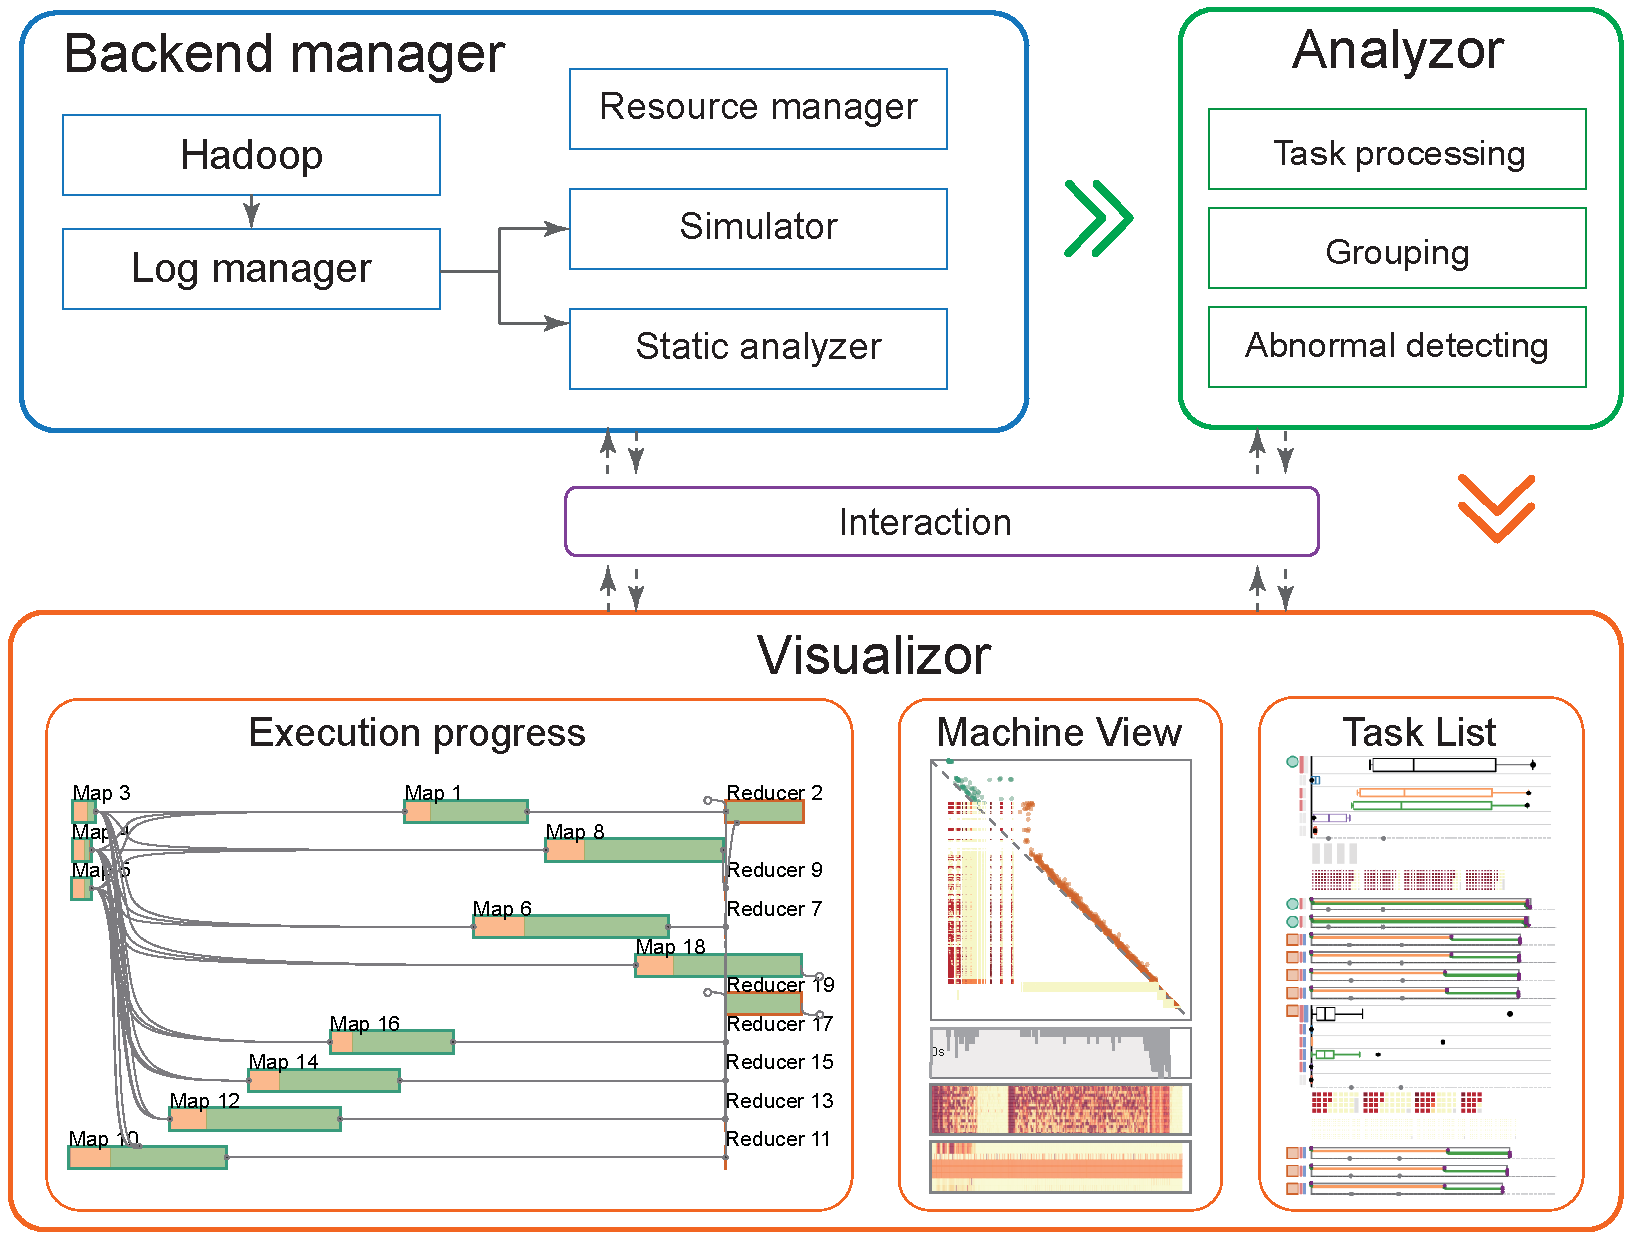
\includegraphics[width=0.49\textwidth]{figures/system/sysdesign.png}
	\vspace{-3mm}
	\caption{$\DQV$ system consists of three major components: backend manager, analyzer and visualizer.}
	\label{fig:sysdesign}
	\vspace{-3mm}
\end{figure}
As shown by Figure~\ref{fig:sysdesign}, $\DQV$ consists of three modules: backend manager, analyzer, and visualizer. 

In our current system, we use Hadoop2.0 as the\textbf{ distributed query engine}. The system can run in three modes: monitoring mode, simulation mode and analytics mode. The monitoring mode directly collect the real-time execution log from Hadoop2.0, then process it and send the result to analyzer. The simulator and log analyzer are linked with log file manager, a module to process and save logs as as structured data form. Log analyzer directly output the strusctured data to the next module. The simulator simulatses the execution progress which allow users to adjust the running speed and explore the dynamic query process. 

The analyzer collects the data from the backend manager and further process them for visualization. 

The visualization module integrates coordinated views to support interactive exploration of and reasoning about the query behaviour at the different perspectives. Execution overview demostrates the execution process in at the vertex level. A new algorithm for the temporal DAG is proposed to visualize the structure and process at the same time. The task view visualize the temporal information of tasks as well as the dataflow relationship among the tasks. The profiling view integrates the task view with the resource status for each machines.  A rich set of interactions are also supported to link different views together.



\section{Data Collection and Preprocessing}

\subsection{Data Collection}
%As shown by figure~\ref{fig:sysdesign}, our analysis pipeline starts from the plan, log, and system performance data collection.
%
%\stitle{Query plan parsing}
%As shown in section~\ref{sec:background}, in Hive, an execution plan is described as a text file involving hundreds to thousands of lines of operations. We parse this file first and generate a directed acyclic graph with the node as the logic vertex and the edge as the data dependencies.
%
%\stitle{Execution log and system performance processing}
%Since the Hadoop execution logs are collected with the tedious system log, we locate the records of interest by detecting the keywords from the pre-defined keyword set and then parse these logs and extract the information.
%Several important information is saved to the local file, including the task id, the logic vertices corresponding to the tasks, the temporal information(start time, duration) of tasks, the temporal information of steps in a task, etc. 

As shown in Figure~\ref{fig:sysdesign}, our visualization pipeline starts from the plan, log, and system performance data collection.

\stitle{Query plan parsing}
As introduced in Section~\ref{sec:background}, in Hive, a logical execution plan is described as a text file that contains hundreds to thousands lines of descriptions. We parse this file and generate a DAG with the vertices being the operators and the edges modeling the data dependencies.

\stitle{Execution log processing}
As Hadoop execution logs are collected from tedious system log, we locate the records of interest by first matching keywords from a pre-defined keyword set and then parsing these logs to extract the required information. The information we save to local files include task id, the logical vertex corresponding to each task, the temporal information (start time, duration) of individual tasks, and the temporal information of the sub-steps in a task. 


\subsection{Data Modeling}

\begin{figure}[t]
	\centering
	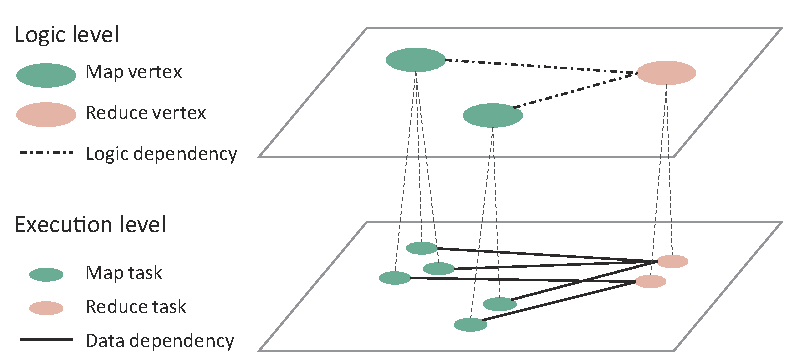
\includegraphics[width=0.42\textwidth]{figures/model/datamodel.pdf}
	\vspace{-3mm}
	\caption{Two-level execution graph.}
	\label{fig:model}
	\vspace{-3mm}
\end{figure}

The data we collected from the backend manager can be modeled as a temporal graph with two levels, i.e., the logical level and the execution-level, which is shown in Figure~\ref{fig:model}. 

%As discussed in section~\ref{sec:background}, the logic level graph indicates the DAG extracted from the execution plan, denoted by $\mathbb{G}_L = (\mathbb{V}_L, \mathbb{D}_L)$, where $\mathbb{V}_L$ is the logic vertex set and the $\mathbb{D}_L$ is logic dependency set between the vertices. The execution-level graph denotes the $\mathbb{G}_E = (\mathbb{T}_E, \mathbb{D}_E)$, where $\mathbb{T}_E$ denotes the set of tasks executed by the the physical machines and $\mathbb{D}_E$ indicates the data dependency set between tasks. 
%If a task $t \in \mathbb{T}_E$ is an physical instance of vertex $v \in \mathbb{V}_L$, we describe this relationship as the form $t \to v$. We also adopt the this description for the relationship between logic dependency $d_L \in \mathbb{D}_L$ and data dependency $d_E \in \mathbb{D}_E$ such as $d_e \to d_L$. Moreover, we use $P(v) = \{t|\forall t \to v\}$ to indicate all tasks which are the physical instances of $\mathbb{V}_L$. 
%A map task $t$ has five steps indicating as an array: $S=<s_{init}, s_{input}, s_{proc}, s_{sink}, s_{spill}>$ and a reduce task have five steps $S=<s_{init}, s_{shuffle}, s_{proc}, s_{sink}, s_{spill}>$. Each step can be modeled by a pair of attributes $<st, d>$ which denotes the start time and durzation. Notice that the different steps of the same task may have overlap in time.
%
%According to section~\ref{sec:background}, each task can be modeled as a sequence of attributes: $t:=<st, d, v, m, S_E>$, where $st$, $d$ and $v$ indicate the \textit{start time}, \textit{duration} and logic vertex of task $t$.  $m$ is the machine executes this task and $S_T$ is the corresponding steps. We use $t.attr$ to indicate the $attr$ of $t$.
%
%The vertex can be modeled as triplet: $v:=<st, d, S_L>$. The start time of $v$ is $v.st=min(\{t.st|t \in P(v)\})$, the duration of vertex $e$ is $v.d=v.st+max(\{(v.st+v.d)|t \in P(v) \})$. The steps $S_L=$ $\{d_{init}, d_{input}, d_{proc}, d_{sink}, d_{spill}\}$ or $\{d_{init}, d_{shuffle}, d_{proc}, d_{sink}, d_{spill}\}$ according to the types, and with a given $v$, $d.attr = sum(\{s.attr| s\in S_L\})$ where $attr \in \{init, input, shuffle, proc, sink, spill\}$. 

The logical level graph is the DAG extracted from the execution plan, denoted by $\mathbb{G}_L = (\mathbb{V}_L, \mathbb{D}_L)$, where $\mathbb{V}_L$ is the logical vertex set and $\mathbb{D}_L$ is logical dependency set between the vertices. The execution level graph is denoted as $\mathbb{G}_E = (\mathbb{T}_E, \mathbb{D}_E)$, where $\mathbb{T}_E$ is the set of tasks executed by the physical machines and $\mathbb{D}_E$ indicates the data dependency set between tasks. 
If a task $t \in \mathbb{T}_E$ is a physical instance of vertex $v \in \mathbb{V}_L$, we describe this relation using $t \to v$. We also apply this description to the relation between logical dependency $d_L \in \mathbb{D}_L$ and psychical dependency $d_E \in \mathbb{D}_E$ and use $d_e \to d_L$. Moreover, we use set $P(v) = \{t|\forall t \to v\}$ to indicate all tasks that are physical instances of logical operator $\mathbb{V}_L$. 
A map task $t$ has five steps and is recorded as an array $S=<s_{init}, s_{input}, s_{proc}, s_{sink}, s_{spill}>$ while a reduce task is recorded as $S=<s_{init}, s_{shuffle}, s_{proc}, s_{sink}, s_{spill}>$. Each step is associated with a pair of time $<st, d>$, which indicates its start time and duration. Note that different steps of the same task may overlap in time due to pipelining.

Each task is modeled as a sequence of attributes $t:=<st, d, v, m, S_E>$, where $st$, $d$ and $v$ indicate the \textit{start time}, \textit{duration} and logical vertex of task $t$.  $m$ is the machine that executes $t$ and $S_T$ is the corresponding steps. We use $t.attr$ to index an $attr$ of $t$. A logical vertex is modeled as a triplet $v:=<st, d, S_L>$. The start time of $v$ is $v.st=min(\{t.st|t \in P(v)\})$, the duration of vertex $v$ is $v.d=v.st+max(\{(t.st+t.d)|t \in P(v) \})$. The steps $S_L=$ $\{d_{init}, d_{input}, d_{proc}, d_{sink}, d_{spill}\}$ or $\{d_{init}, d_{shuffle}, d_{proc}, d_{sink}, d_{spill}\}$ according to the type of the vertex (i.e., map or reduce). For a given $v$, $d.attr = sum(\{s.attr| s\in S_L\})$ where $attr \in \{init, input, shuffle, proc, sink, spill\}$. 
\section{Visualization design}
\subsection{Query execution overview}
\subsubsection{Execution plan view}
\subsubsection{Execution progress view}
\subsection{Task view}
\subsection{System profiling visualization}
\subsection{Linkage and interactions}
\section{Evaluation}
\subsection{Case study}
We collaborated with the domain experts to demonstrate the effectiveness of $\DQV$ by analyzing several real world cases which are slower than our exception.

\subsubsection{Identify the hardware bottleneck}
The first case is executed on a cluster with 5 nodes and run around 623 seconds. The execution plan is shown as the Figure~\ref{fig:teaser}(A).

When exploring the execution with $\DQV$, we find that in the progress view, it is obvious Map1(Figure~\ref{fig:teaser}(B1)) significantly run longer than the duration of other vertices. On the other side, the Reducer2, a subsequent vertex of Map1, finished in a very short time after Map1 is finished. Reducer is followed by a sequence of short reduce vertices(shown as Figure~\ref{fig:teaser}(B3)) which are quickly executed after that. 
From this pattern, we guess the bottleneck should be related Map1, several abnormal tasks may lead to the long execution time of Map1. We hover the mouse on it to highlight the associated tasks as blue color in the Distribution View.
In the summary distribution view, we can see there are two task groups which are distributed far away from each other (shown as Figure~\ref{fig:teaser}(C5, C6)). 
By checking the blue-colored tasks on the machine views through cross-view linking, we find the tasks at the left top corner are dispatched on the machine dbg14, dbg16, dbg19 and dbg20. But the tasks on the right bottom corner are only executed on machine dbg18. Moreover, it seems that dbg18 only executes very few tasks in this case. 
We further check the cluster and notice that something wrong with the network of dbg18, thus the tasks assigned to it are delayed and executed very late, leading to the overall long duration of the query execution. In the exploration of summary view, we can find the these tasks of Map1 provides the data to several tasks of Reducer2, shown as the Figure~\ref{fig:teaser}(C1), which also verifies our assumption. 

In addition to Map1, we notice another vertex Map24 also have a very long duration. When we click to mark the tasks of Map24 (these tasks are colored as purple), we find that none of them are executed on dbg18. So we guess dbg18 is not the only reason results in the slow query. At the same time, there is one task run with a very long time (shown as Figure~\ref{fig:teaser}(C2)) on the machine dbg19. Moreover, the dbg19 executes far fewer tasks than the machine dbg14, dbg16 and dbg20, but these tasks tends to have longer duration. By exploring the performance view, we find the CPU usage view of dbg19 has large piece of red color region, indicating the the CPU is more busy than the other machines(shown as Figure~\ref{fig:teaser}(C3)). We further explore the system log and find there are several computing-bounded programs are executed on dbg19 at the same time which takes the computing resource thus making these query tasks very slow.

\begin{figure}[t]
	\centering
	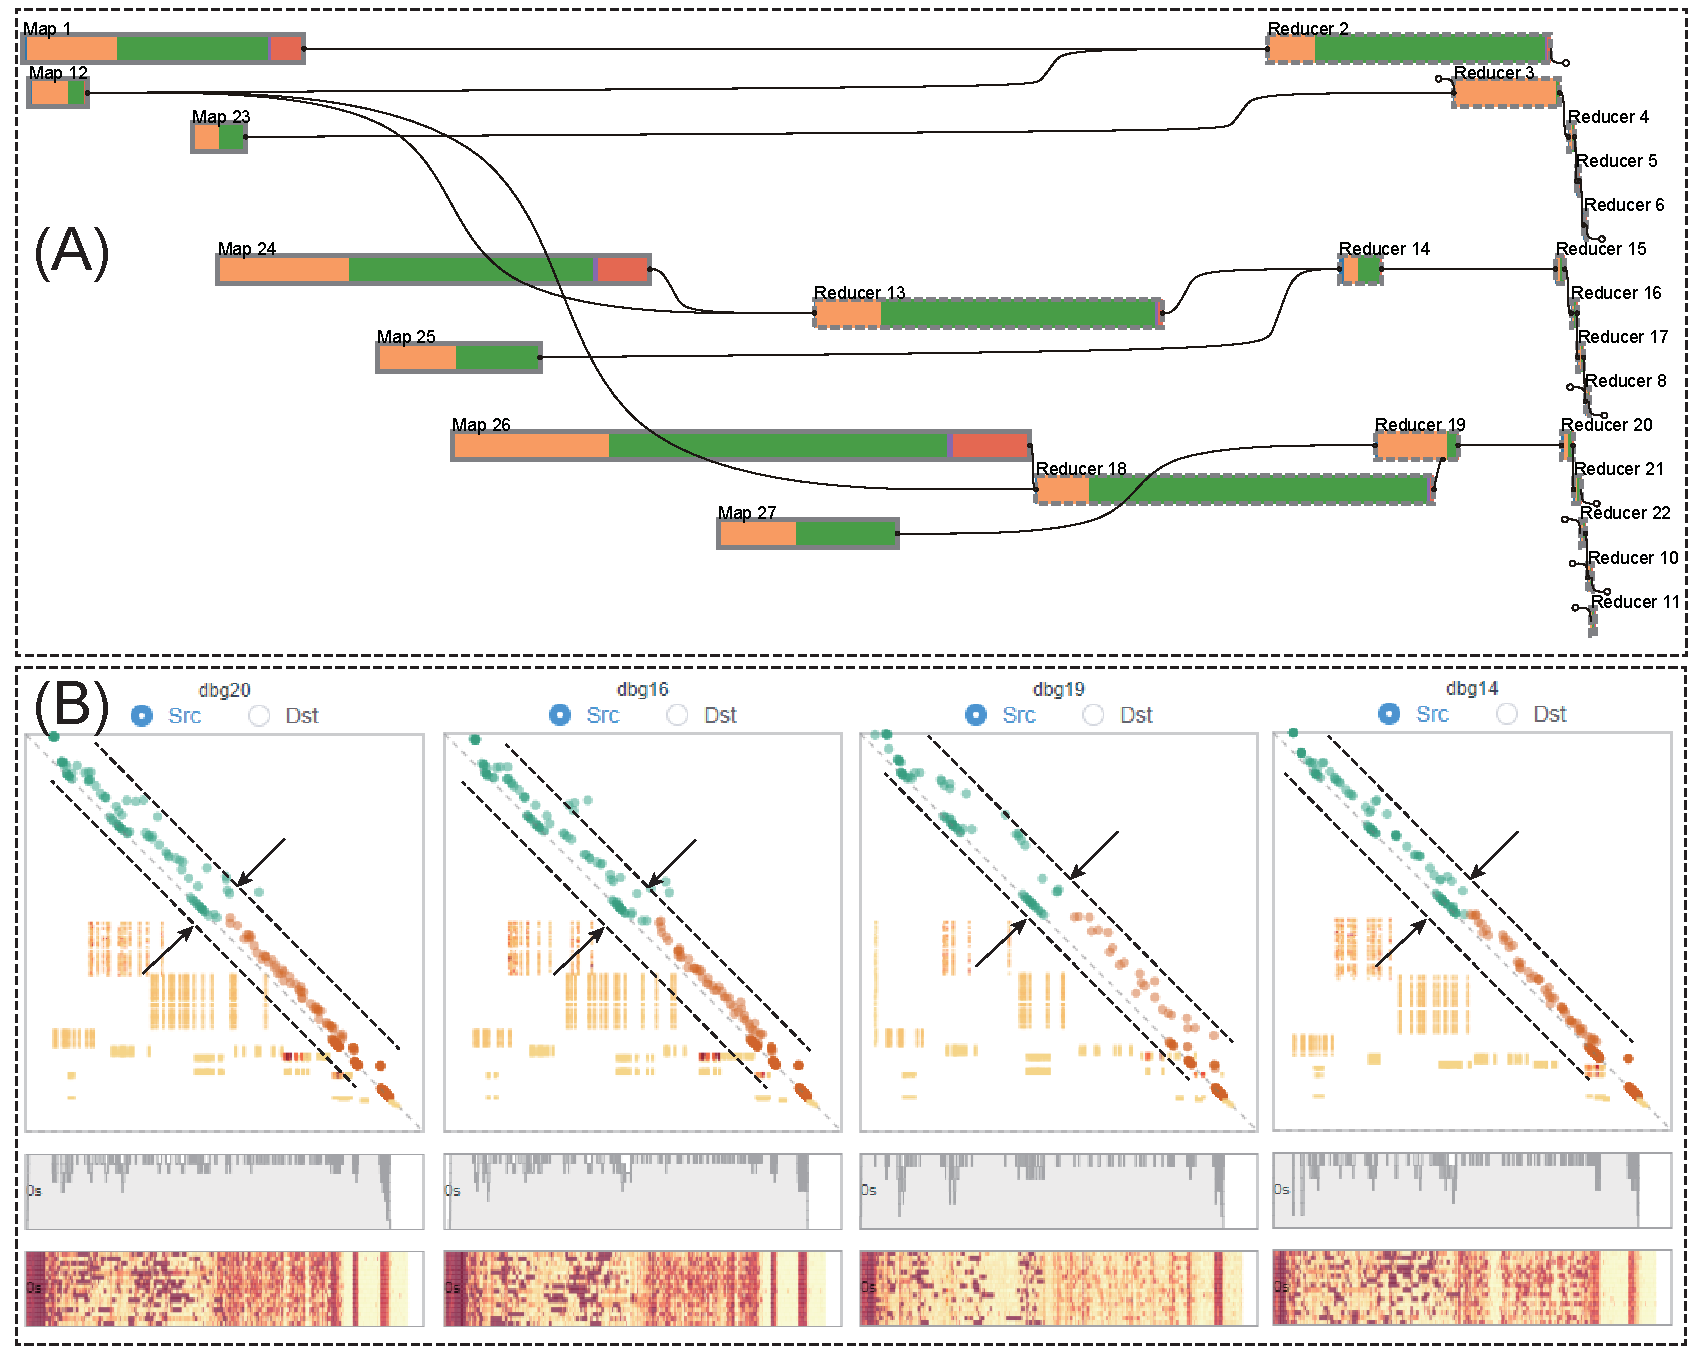
\includegraphics[width=0.45\textwidth]{figures/case_study/CaseStudy1.pdf}
	\vspace{-3mm}
	\caption{Re-execute the query after removing a unhealthy node and stop the CPU-bound programs.}
	\label{fig:casestudy1}
	\vspace{-3mm}
\end{figure}


To address this problem, we directly remove the node dbg18, stop the other programs run on server dbg19 and re-execute the same query. The query is finished with 200s. In the progress view, we find the duration of both vertex Map1 and Map24 are greatly reduced shown as Figure~\ref{fig:casestudy1}(A). We also find that in the distribution view, all the tasks are distributed close to the diagonal line indicating that they are all executed within the small time range Figure~\ref{fig:casestudy1}(B). Moreover, the CPU performance view shows that all the CPUs on different server have the balanced performance. 

\subsubsection{Diagnose the task failure}



\begin{figure*}
	\vspace{2mm}
	\centering
	\small
	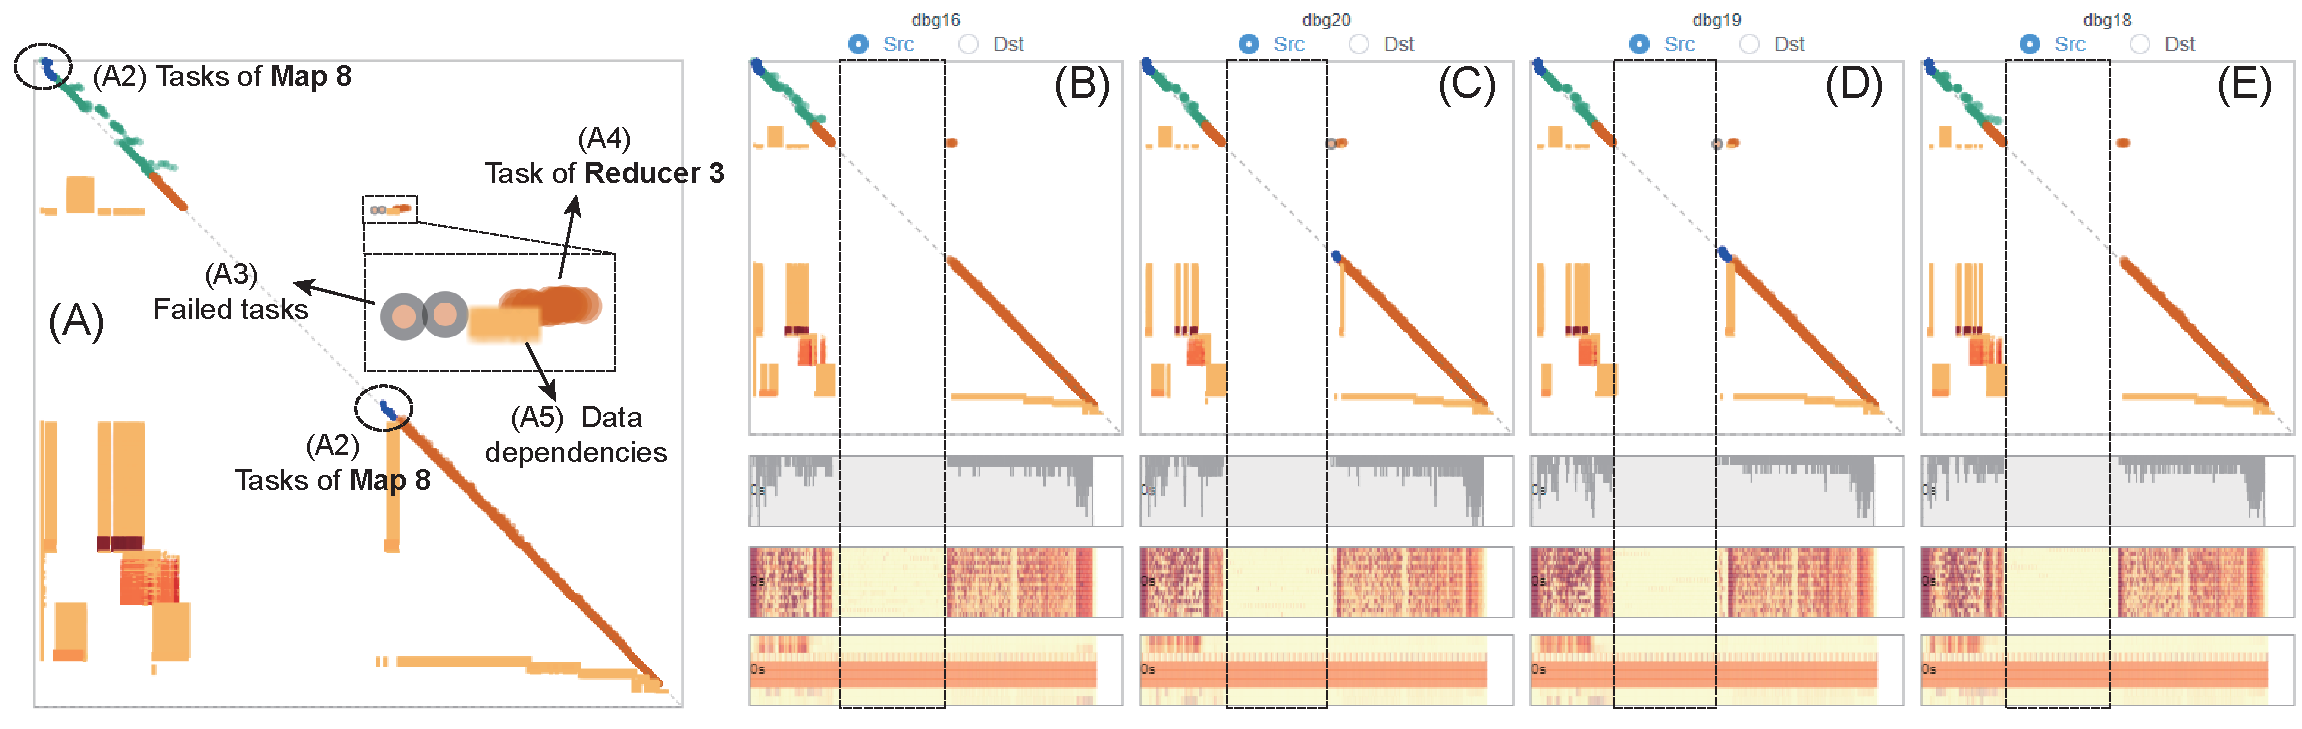
\includegraphics[width=2\columnwidth]{figures/case_study/CaseStudy2.pdf}  

	%\vspace{-3mm}
	\caption{Analyze the task failure.} 
	\label{fig:casestudy2}

\end{figure*}


The second case runs on the cluster with four nodes. As show by the summary view,  we notice that there are two tasks failed during the execution. The expert wants to know how why these tasks are failed. By observing the performance view, we notice during the execution of the failed tasks, the all the machine run the maximum number of tasks but the usage of their CPU, memory and network are not fully used, which indicating these tasks take the quota of the works but do nothing. but cannot finished until two tasks are abandoned.
***

\subsubsection{Understand the data skew}

\begin{figure}[t]
	\centering
	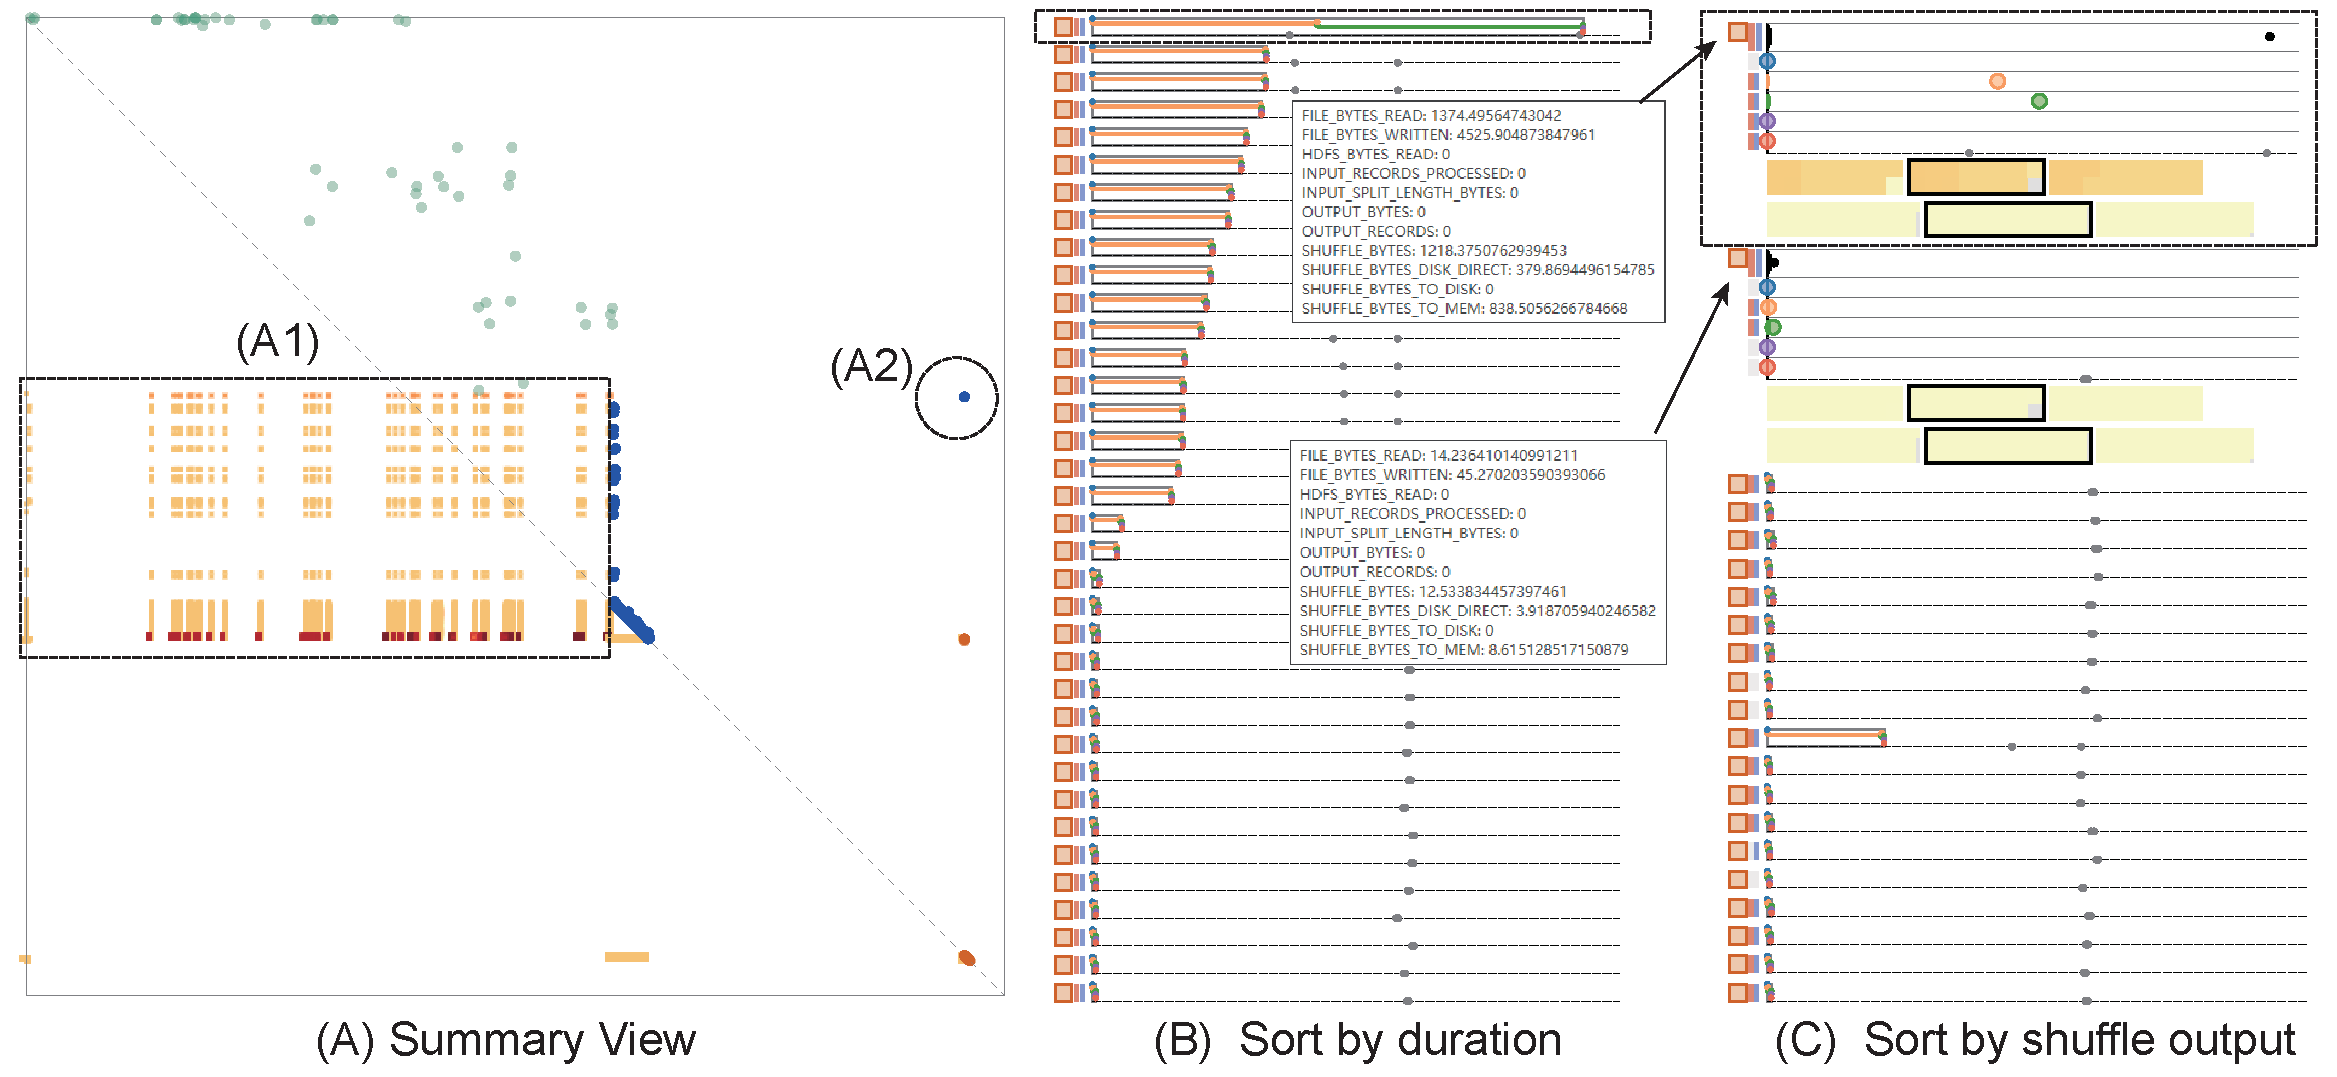
\includegraphics[width=0.45\textwidth]{figures/case_study/CaseStudy3.pdf}
	\vspace{-3mm}
	\caption{Detect the data skew.}
	\label{fig:casestudy3}
	\vspace{-3mm}
\end{figure}

\input{sections/user}
\section{Conclusion}
In this paper, we propose $\DQV$, an interactive visual system for Hive query execution analysis. 
$\DQV$ consists of three linked views which transfer the multi-level progress data into different visual forms according to the analyzing requirements, including:
1) a space-efficient algorithm to layout the TDAG, which displays the progress and the clear topology structure simultaneously; 
2) a novel visual encoding method to visualize the complex task dependencies and task distribution, system performance is also integrated with it to allow users to reason the query patterns; 
3) a task view for individual task analysis. Three case studies about the query execution understanding, resource bottleneck detection and query debugging as well as two user interviews show our system can be helpful in real-world practices.


%% if specified like this the section will be committed in review mode
% \acknowledgments{
% The authors wish to thank A, B, and C. This work was supported in part by
% a grant from XYZ (\# 12345-67890).}

%\bibliographystyle{abbrv}
\bibliographystyle{abbrv-doi}
%\bibliographystyle{abbrv-doi-narrow}
%\bibliographystyle{abbrv-doi-hyperref}
%\bibliographystyle{abbrv-doi-hyperref-narrow}

\bibliography{template}
\end{document}

